\chapter{Cinématique II: Le mouvement}
\label{sec:cinediff}





Cinématique:

%%%%%%%%%%%%%%%%
\begin{equation}
\text{Cinématique directe:}  \quad \col{r} = f\left( \, \col{q} \, \right)  \quad  \text{inverse:} \quad \col{q} = f^{-1}\left( \, \col{r}  \, \right) 
\end{equation}
%%%%%%%%%%%%%%%



Cinématique différentielle:


%%%%%%%%%%%%%%%%
\begin{equation}
\text{Cinématique différentielle directe:} \quad \col{\dot{r}} = J\left( \, \col{q} \, \right) \, \col{\dot{q}}   \quad \text{inverse:} \quad \col{\dot{q}} = J^{-1}\left( \, \col{q} \, \right) \, \col{\dot{r}}
\end{equation}
%%%%%%%%%%%%%%%

%%%%%%%%%%%%%%%%
\begin{equation}
\text{Matrice Jacobienne:} \quad J\left( \col{q} \right) = \frac{\partial \col{r}}{\partial \col{q}}
\end{equation}
%%%%%%%%%%%%%%%%

%%%%%%%%%%%%%%%%
\begin{equation}
\text{Dérivées en chaînes:} \frac{d \col{r}}{dt} = \left( \frac{\partial \col{r}}{\partial \col{q}} \right) \frac{d \col{q}}{dt} 
\end{equation}
%%%%%%%%%%%%%%%%


\subsection{Exemple: Cinématique différentielle d'un robot à deux joints}


%%%%%%%%%%%%%%%%%%%%%%%%%%%%%%%%%%%
\begin{align}
\col{r} &= \left[ \begin{array}{c} x \\ y  \end{array} \right]  = \left[ \begin{array}{c} 
-l_1 c_1 + l_2 c_{12} \\ 
 l_1 s_1 + l_2 s_{12}  
\end{array} \right] 
\end{align} 
%%%%%%%%%%%%%%%%%%%%%%%%%%%%%%%%%%%
avec
%%%%%%%%%%%%%%%%%%%%%%%%%%%%%%%%%%%
\begin{align}
c_1    &= \cos( q_1 ) \\
s_1    &= \sin( q_1 ) \\
c_{12} &= \cos( q_1 + q_2 ) \\
s_{12} &= \sin( q_1 + q_2 )
\end{align} 
%%%%%%%%%%%%%%%%%%%%%%%%%%%%%%%%%%%
Dérivation:
%%%%%%%%%%%%%%%%%%%%%%%%%%%%%%%%%%%
\begin{align}
\dot{\col{r}} &= \frac{d\col{r}}{dt} = \left[ \begin{array}{c} \dot{x} \\ \dot{y}  \end{array} \right]  = \left[ \begin{array}{c} 
-l_1 s_1 \dot{q}_1 - l_2 s_{12}( \dot{q}_1 + \dot{q}_2 ) \\ 
 l_1 c_1 \dot{q}_1 + l_2 c_{12}( \dot{q}_1 + \dot{q}_2 )  
\end{array} \right] \\
\dot{\col{r}}  &= 
\underbrace{ \left[ \begin{array}{c c } 
-l_1 s_1 - l_2 s_{12} & - l_2 s_{12} \\ 
 l_1 c_1 + l_2 c_{12} &   l_2 c_{12}
\end{array} \right]  }_{ J(\col{q}) } 
\underbrace{ \left[ \begin{array}{c} 
\dot{q}_1 \\ 
\dot{q}_2 
\end{array} \right]}_{ \dot{\col{q}} } \\
\dot{\col{r}}  &= J(\col{q}) \dot{\col{q}}
\end{align} 
%%%%%%%%%%%%%%%%%%%%%%%%%%%%%%%%%%%



\subsection{Robot hyper-redondant}

%%%%%%%%%%%%%%%%%%%%%%%%%%%%%%%%%%%
\begin{align}
m > n
\end{align} 
%%%%%%%%%%%%%%%%%%%%%%%%%%%%%%%%%%%

%%%%%%%%%%%%%%%%%%%%%%%%%%%%%%%%%%%
\begin{align}
m &= dim(\col{q}) = \quad\text{Nombre de DDL du robot} \\
n &= dim(\col{r}) = \quad\text{Coordonnées de l'espace de la tâche} 
\end{align} 
%%%%%%%%%%%%%%%%%%%%%%%%%%%%%%%%%%%

Cinématique différentielle:
%%%%%%%%%%%%%%%%%%%%%%%%%%%%%%%%%%%
\begin{align}
\left[ \begin{array}{c}  \\ \dot{\col{r}} \\ \\
\end{array} \right]_{m \times 1}
&= 
\left[ \begin{array}{c c c c c} 
&&&&\\
&& J(\col{q}) &&\\
&&&&
\end{array} \right]_{m \times n}
\left[ \begin{array}{c} 
\\ \\ \dot{\col{q}} \\ \\ \\
\end{array} \right]_{n \times 1}
\end{align} 
%%%%%%%%%%%%%%%%%%%%%%%%%%%%%%%%%%%


Cinématique inverse:
%%%%%%%%%%%%%%%%%%%%%%%%%%%%%%%%%%%
\begin{align}
\left[ \begin{array}{c}  \\ \\ \dot{\col{q}} \\ \\ \\
\end{array} \right]_{n \times 1}
&= 
\left[ \begin{array}{c c c} 
&&\\ &&\\ & J^{\#} & \\&& \\ &&
\end{array} \right]_{n \times m}
\left[ \begin{array}{c} 
\\ \dot{\col{r}} \\ \\
\end{array} \right]_{m \times 1} + 
\left[ \begin{array}{c c c c c} 
&&&&\\ &&&&\\ && I - J^{\#}J && \\&&&& \\ &&&&
\end{array} \right]_{n \times n}
\left[ \begin{array}{c} 
\\ \\ \col{\Psi} \\ \\ \\
\end{array} \right]_{n \times 1}
\end{align} 
%%%%%%%%%%%%%%%%%%%%%%%%%%%%%%%%%%%
avec
%%%%%%%%%%%%%%%%%%%%%%%%%%%%%%%%%%%
\begin{align}
J^{\#} = J^T\, (JJ^T)^{-1}
\end{align} 
%%%%%%%%%%%%%%%%%%%%%%%%%%%%%%%%%%%








%%%%%%%%%%%%%%%%%%%%%%%%%%%%%%%%%%%%%%%%%%%%%%%%%%%%%%%%%%%%%%
\newpage
\section{Vitesse et dérivée d'un vecteur position}



%%%%%%%%%%%%%%%%%%%%%%%%%%%%%%%%%%%
\subsection{Référentiel} 
Un référentiel est un solide ou un ensemble de points par rapport auquel un observateur qui mesure un mouvement est fixe. Une position ou un mouvement ne peut être défini par rapport au vide et il n'y a pas de référentiel absolu, le choix du référentiel est donc un choix arbitraire de point de vue. Il est à noter que \textbf{contrairement au choix d'un repère, le choix du référentiel influence "la physique" du problème}, par exemple l'énergie cinétique d'un objet n'est pas la même selon le référentiel alors que cette quantité est indépendante du système de coordonnées. Un référentiel dit inertiel ou Galiléen (vitesse et orientation constante) est préférable si on souhaite éventuellement appliquer les équations de Newtons, car des facteurs correctifs (ex.: la force centrifuge) doivent être ajoutés aux équations dynamiques si un référentiel non-inertiel est utilisé. La notion de référentiel est critique pour le calcul de vitesses et accélérations, mais on peut en faire abstraction pour les problèmes de cinématique et statique qui n'impliquent pas la notion d'évolution dans le temps. 


%%%%%%%%%%%%%%%%%%%%%%%%%%%%%%%%%%%%%
\subsection{Référentiel vs. repère}
Pour décrire le mouvement d'un objet, les concepts de référentiel, origine et base vectorielle sont important à distinguer. En quelques mots, un \textbf{référentiel} est un point de vue utilisé pour décrire un phénomène, une \textbf{origine} c'est un point par rapport auquel les mesures de position sont faites et une \textbf{base} vectorielle représente l'orientation du système d'axe utilisé. Ces trois éléments peuvent être choisi indépendamment.  Ensuite, un \textbf{repère} c'est la combinaison d'une base et d'une origine. Par exemple, pour décrire la position d'un bateau, typiquement le référentiel utilisé serait la Terre, l'origine des mesures de position pourrait être le port le plus près, et la base pour exprimer cette position serait le système d'axe nord-sud/est-ouest. Il est important de noter que tous ces choix sont indépendants et les confondre est une source d'erreur courante en cinématique. Le reste de cette section discute de ce qui les distingue.

%%%%%%%%%%%%%%%%%%%%%%%%%%%%%%%%%%%%%%%%%%%%%%%%%%%%%%%%%%%%%%%%%%%%%%%%%%%%%
\begin{figure}[H]
	\centering
		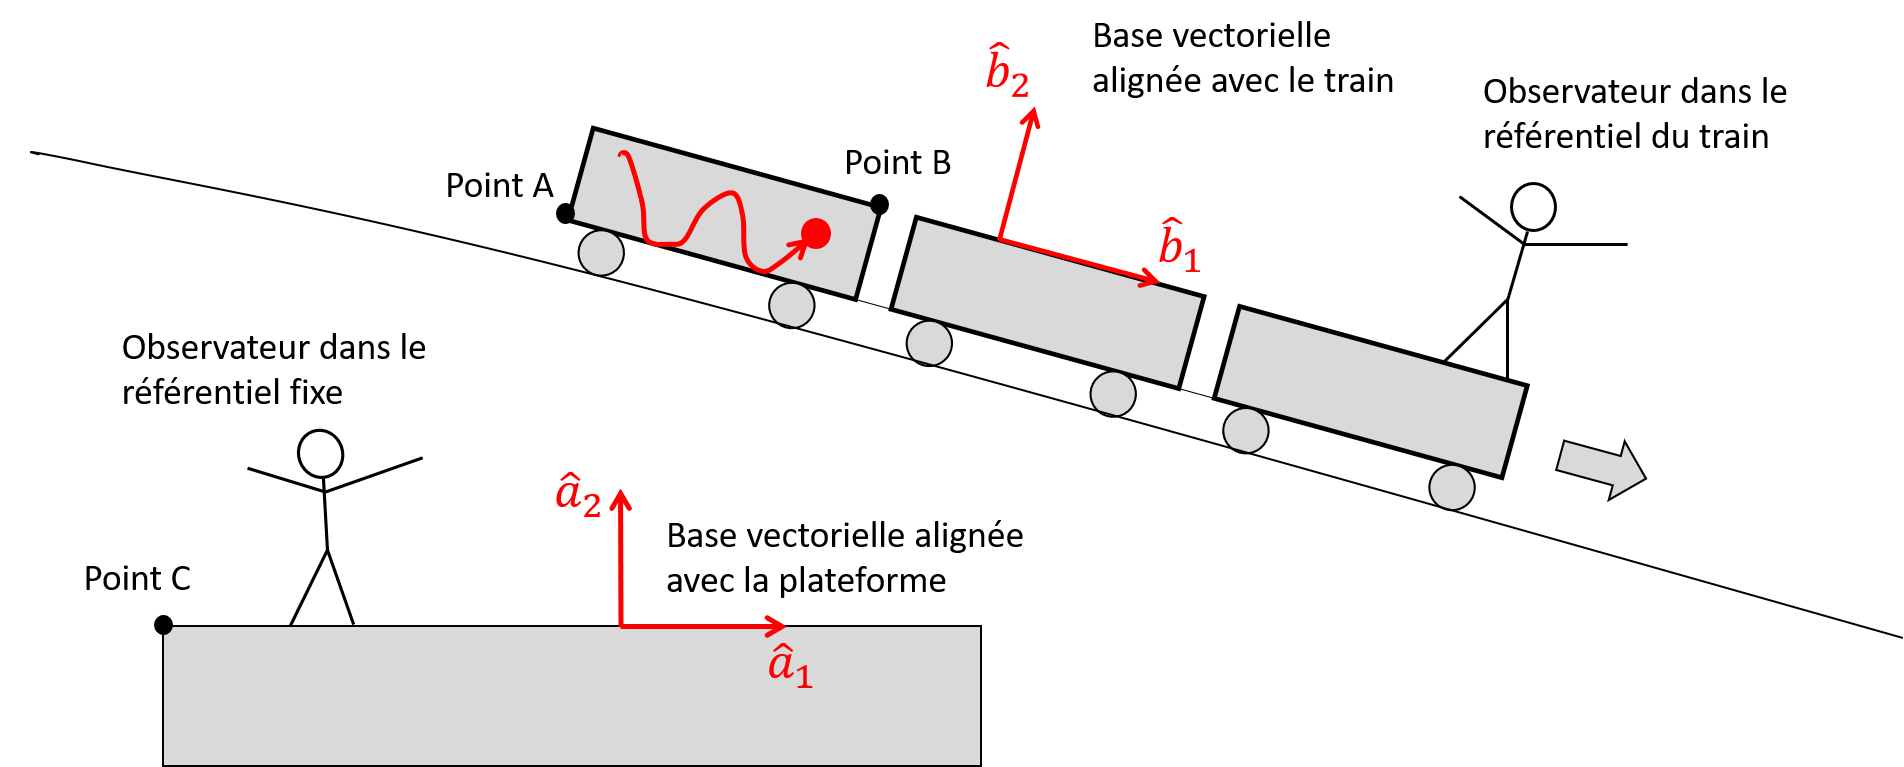
\includegraphics[width=0.90\textwidth]{train.png}
	\caption{Exemple de référentiels, points d'origine et bases vectorielles}
	\label{fig:train}
\end{figure}
%%%%%%%%%%%%%%%%%%%%%%%%%%%%%%%%%%%%%%%%%%%%%%%%%%%%%%%%%%%%%%%%%%%%%%%%%%%%%%%

La figure \ref{fig:train} illustre ces concepts par un exemple où un train descend une pente à vitesse constante et un ballon rebondit sur le sol du troisième wagon. Deux bases vectorielles sont définies, une alignée avec l'horizontale et une alignée avec le train. Plusieurs points d'origine pour les mesures de position sont aussi disponibles. Finalement, deux référentiels sont définis, un référentiel attaché à la Terre (fixe) et un référentiel qui est attaché au train. Les coordonnées d'un vecteur-colonne qui décris la position du ballon:
%%%%%%%%%%%%%%%%%%%%%%%%%%%%%%%%%%%%%
\begin{equation}
\col{r}_{Ball} = \left[ \begin{array}{c} r_1 \\ r_2 \end{array} \right]
\end{equation}
%%%%%%%%%%%%%%%%%%%%%%%%%%%%%%%%%%%%%
sont illustrés pour différents choix d'origine et de base vectorielle, lorsque que le référentiel fixe est utilisé (figure \ref{fig:refex1}) et lorsque que le référentiel du train est utilisé (figure \ref{fig:refex2}). Il est à noter que les points d'origine sont ici fixés à la Terre lorsque le référentiel fixe est utilisé, et fixés au train lorsque que le référentiel du train est utilisé. Comme illustré pour cet exemple, \textbf{un changement d'origine est analogue à une translation} de la trajectoire, \textbf{un changement de base vectorielle est analogue à une rotation} de la trajectoire, et \textbf{un changement de référentiel est ici analogue à une dilatation} de la trajectoire dans la direction $\hat{b}_1$, qui correspond à la direction de la vitesse du train. 

%%%%%%%%%%%%%%%%%%%%%%%%%%%%%%%%%%%%%%%%%%%%%%%%%%%%%%%%%%%%%%%
\begin{figure}[htpb]
				%\vspace{-10pt}
        \centering
        \subfloat[Repère $\{ A, \hat{a}_1, \hat{a}_2, \hat{a}_3\}$]{
				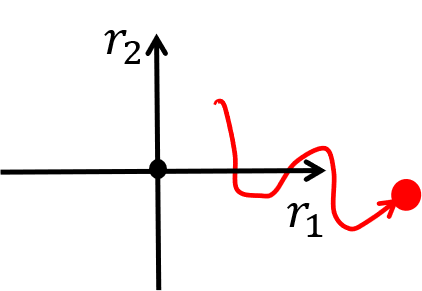
\includegraphics[width=0.23\textwidth]{ref_fixe_r_a_A.png}
				} \hspace{20pt}
				\subfloat[Repère $\{ B, \hat{a}_1, \hat{a}_2, \hat{a}_3\}$]{
				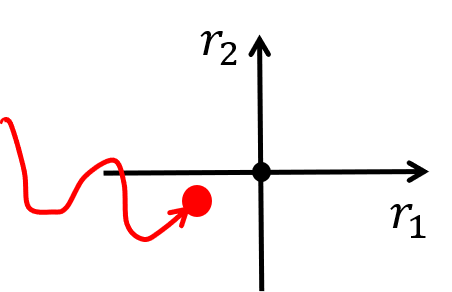
\includegraphics[width=0.24\textwidth]{ref_fixe_r_a_B.png}
				} \hspace{190pt}
				\subfloat[Repère $\{ A, \hat{b}_1, \hat{b}_2, \hat{b}_3\}$]{
				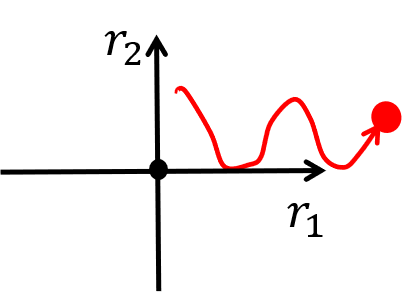
\includegraphics[width=0.22\textwidth]{ref_fixe_r_b_A.png}
				} \hspace{20pt}
				\subfloat[Repère $\{ B, \hat{b}_1, \hat{b}_2, \hat{b}_3\}$]{
				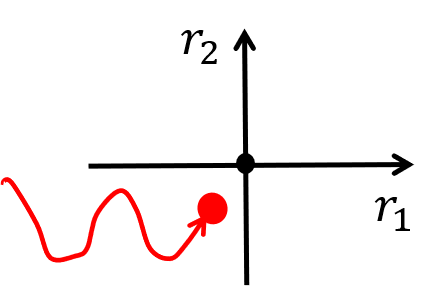
\includegraphics[width=0.24\textwidth]{ref_fixe_r_b_B.png}
				}
        \caption{Trajectoire du ballon avec un repère attaché au \textbf{référentiel fixe}}
				\label{fig:refex1}
\end{figure}
%%%%%%%%%%%%%%%%%%%%%%%%%%%%%%%%%%%%%%%%%%%%%%%%%%%%%%%%%%%%%%%%%

%%%%%%%%%%%%%%%%%%%%%%%%%%%%%%%%%%%%%%%%%%%%%%%%%%%%%%%%%%%%%%%
\begin{figure}[htpb]
				%\vspace{-10pt}
        \centering
				\subfloat[Repère $\{ A, \hat{a}_1, \hat{a}_2, \hat{a}_3\}$]{
				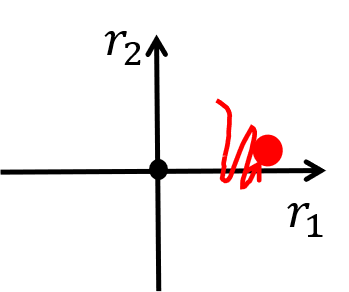
\includegraphics[width=0.22\textwidth]{ref_train_r_a_A.png}
				} \hspace{20pt}
				\subfloat[Repère $\{ B, \hat{a}_1, \hat{a}_2, \hat{a}_3\}$]{
				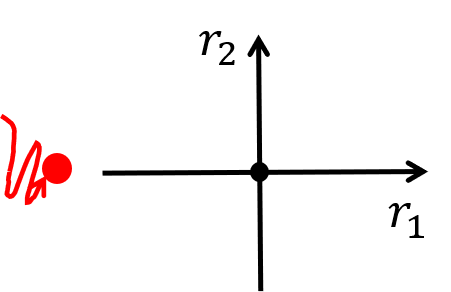
\includegraphics[width=0.25\textwidth]{ref_train_r_a_B.png}
				} \hspace{190pt}
				\subfloat[Repère $\{ A, \hat{b}_1, \hat{b}_2, \hat{b}_3\}$]{
				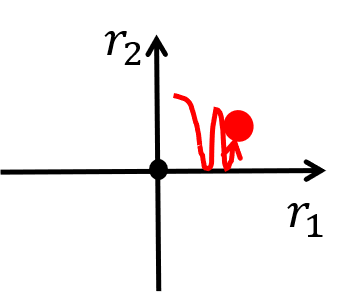
\includegraphics[width=0.22\textwidth]{ref_train_r_b_A.png}
				} \hspace{20pt}
				\subfloat[Repère $\{ B, \hat{b}_1, \hat{b}_2, \hat{b}_3\}$]{
				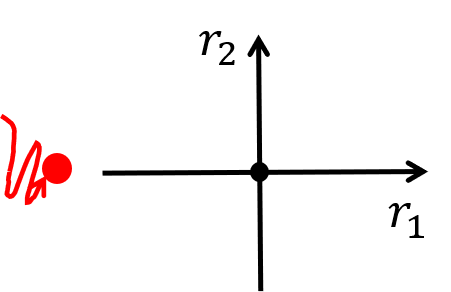
\includegraphics[width=0.25\textwidth]{ref_train_r_a_B.png}
				}
        \caption{Trajectoire du ballon avec un repère attaché au \textbf{référentiel du train}}
				\label{fig:refex2}
\end{figure}
%%%%%%%%%%%%%%%%%%%%%%%%%%%%%%%%%%%%%%%%%%%%%%%%%%%%%%%%%%%%%%%%%

